%=======================================================================================%
% the main points of this introduction are 
% outline the complexity of biological systems for physicists
% 	> even though our theoretical models should preidct everything on the energy and length scales of biology we can't because of their heterogeneity.
%   > Give examples of the heterogenaity 
% Give some points on the history of molecular biophysics  
%   >  Hodgkin-Huxley Models
%   > Gramicidin 
% Point out how Cystic Fibrosis is an expression of this progression, going from genotype to phenotype using an ion channel to teach us biophysics. 
% conclusion.
\pagenumbering{arabic}
\chapter{Introduction: A Philosophy on Physical Biology}
\setcounter{page}{1}
\label{chap:intro}
\chapquote{Whatever complexity means, most people agree that biological systems have it. -Frauenfelder and Wolynes \cite{frauenfelder1994} } {}
\section{Thesis and Chapter Summary}
This thesis seeks to apply a molecular philosophy on biophysics to demonstrate its ability to elucidate pressing problems in biology and medicine. In particular, we will look at how knowledge of the molecular details in the function of a protein ion channel has important cellualr functions.

In this first short chapter we will quickly build a philosophy of how to look at biology through the lens of a physicist. First we will outline what the goal of a physicist is, to create abstract formalisms which can be used to model the natural world. We will then observe what makes the construction of such analogies so dififcult in biology and how a specific set of examples, namely ion channels, allow us to work upward and speculate at the function of more complex biological systems such as cells. 

Chapter \ref{chap:methods} describes in some detail the chemical and numerical simulation techniques we used to study the CFTR protein system.  Chapters \ref{chap:i37r}, \ref{chap:r352q}, \ref{chap:s945l} and \ref{chap:opening} demonstrate how a diverse application of these techniques can be used to discover unique modes of misfunction introduced by a mutation and in combination with \textit {in vitro} cellular techniques, prove that these mutations can be rescued by existing drug regimens.  Finally, chapter \ref{chap:conclusion} argues for a physical model for the action of cystic fibrosis .


\section{What is Physics?}
Personally, I have always described physics answers along the lines of "the study of the movement of energy within a system" or when I was in high school "The study of how things move". Although adequate for a layman these might obscure the process of creating physical models that make it such a powerful tool. Physical theories rely on the conceptualisation of some causal unit in a system and then use mathematics to scale up the behaviour of that unit to make predictions about measurable phenomena. This is what makes physics feel like the most "fundamental" of the sciences

This might take a few different forms at different scales. Examples might be.

Newton's laws of gravitation to explain the movements of the celestial bodies in the solar system. 

Einstein's theories employing Reimannian geometry to track the motions of galaxies and black holes.

The approximation of atoms as hard spheres used to derive the macroscopic behaviour of gasses.

The schrodinger wave function to find the structure of atoms, which can then be integrated further up to find their macroscopic organisations. In chapter \ref{chap:methods} I'll walk you through how we use these laws to model biomolecular dynamics.  

The field of biophysics has an interesting origin. Erwin Schroedinger wrote an essay titled "What is Life?" This remarkable work, written in  1944 before the discovery of DNA or the maturation of information theory speculates from first principals in thermodynamics and quantum mechanics, the nature of life at the atomic level. The most remarkble thing about this essay is how much the author gets right. The observation that since organisms exist at high (?) temperatures the phyical encoding of their genome must be chemical in nature, as energy barriers lower than that of chemistry would be oblated by at physiological temperatures. Schroedinger posits the existence of what he  calls an "aperiodic crystal". He was right, this crystal just happened to be one dimensional. This allegory is an example of how physcial principals can in fact be used to make testable, far reaching predictions about fundamental biology. The details may simply be more difficult since it is harder to capture the heterogeneous details inside cells.

Biological systems exhibit such a problem for the physicist because unlike the above problems it is extremely hard to pick out a fundamental unit to even begin our upwards journey. An evolutionary biologist might say to choose the "gene" but this is actually far too high in our spatial heirarchy already. Really, a gene is only meaningful to the dance of life if it has partners to dance with. 

A coil of DNA in water doesn't really do much in solution except decay without machinary that can preserve, read, translate and replicate it. The gene is an emergent property, we have to go deeper. 

So, what are the gene's partners? 

A slew of biological machinary that mostly take the form of proteins. These proetins are a special case of chemistry, with many observable functions. Their sequence is  coded by the DNA in something reminiscent of a strange loop \cite{hofstadter2007}. 

This self referential loop is one of the reasons biology is so difficult. Since we know that this strange loop is kicked off by atomic interactions we will start there. As we are taking a physical, pragmatic approach here it would make sense to begin with the protein, after all, they stave off the march of entropy constantly trying to eat up all of your cells. It also just so happens that they are much easier to understand computationally since their motions are faster and more flexible. 

The first level sub cellular organisation is perhaps the most intimdating first step for me personally after spending 4 years simulating a single protein. Glimpsing the complexity within a single one of these molecules has been one of the most existential experiences of my life but the knowledge that there are astronomical numbers of these things inside me all of the time terrifies me.

It is hoped that illustrating the monumental task in both intellectual effort and resources of incrementally increasing the understanding of a single protein amongst the 23000 or so encoded in our genome will give the reader and understanding of how we might continue our quest to understand the molecular dance that plays within all of us.  
 
%Somewhere on the scale between a single protein and a single cell this is what we consider "life". We have single unicellular organisms but we don't have uniproteomic organisms. So the fundamental length scale of life is somewhere between $10^{-10}m$ and $10^{-3}m$. This is the first loop in our strange loop.

After this things start to run away from me with my handful of GPUs and limited patience. So in this thesis we will only discuss single proteins.
%Biological strange loops would not seem to be as self similar as the clean nice logics in the strange loop of the Godelian knot. Why is this?

\section{The Physics Inside your Cells}
\chapquote{}{}

\vskip 0.5cm

Why can't I  write down an equation which will tell me how long I will live? Or how tall I will grow?

This might seem like an inane question but if you asked a physicist how much power it would take to ionise a gas or how long it will take a black hole to evaporate and they will have highly accurate models at the ready to answer easily. 

What makes the first set of questions so much more difficult to answer?

Our current physical theories have sufficient accuracy at the energy and length scales of biology that we can accuarately model every phenomenon inside a living being\cite{carroll2021}. So why are living systems so hard to study for theorists?

The complexity of biology does not arise from complex interactions. As we will see in \ref{chap:methods} the interactions between atoms within living things is surprisngly simple. Rather, the complexity arises from the simple interactions between many diverse components. Inside cells we find proteins, lipids, solvents, salts each with their own properties. Biophysics distinguishes itself from more tradiational physics as it considers systems that are highly heterogeneous and anisotropic. For simple physical systems the physicist can draw on conceptual tools such as a mass on a spring or a gas of hard spheres which can be extremely successful in explaining many phenomena. 

For biological systems there appears to be too much complexity for such analogies to have the same level of success. 

The heterogeneity of biology is easy to observe. If you look at your arm, you will notice hair, pores, dry skin, dead skin, perhaps even tendons and muscles twitching beneath the surface. That skin is itself made of layers there are two more layers to your skin with different functions and composition. If you were to take a single cell from any of those layers and stain it to distinguish features in an electron microscope you would notice all sorts of complex structures and the size and number of these structures would vary depending on where you took the cell from in the body. Within and between each those structures is a salty, wet dance of molecules large and small. This heterogeneity on length scales hints at the reasons behind biology's physical complexity. Plasma physicists may use the same mathematical tools to describe materials as diverse as the dense stellar core to the sparse intergalactic nebulae these span 28 orders of magnitude in density \cite{chen2018}. Would that we were so lucky in biology. We struggle to apply same physical models to deal with phenomena across a single order of magnitude.  

Thus, in order to move towards more predictive theories of biology it is necessary to consider much more of the fundamental physical processes occurring within biological systems than simply searching for statistical trends. One form of this from fundamentals approach is the simulation of every atom in a biological system. Although computationally expensive, this approach has been proven necessary due to the heterogeneous nature of biological systems \cite{moy2000, corry2000a}. We can sadly get away with very little idealisation when it comes to the molecular details of proteins.

One of the things we're trying to do with molecular dynamics is fill in the gap left by the sequence->function paradigm which is internalised in current understandings of molecular biology. We usually talk about how the sequence of the gene defines its function because it gives the protein its structure but really there is a considerably larger amount of regulatory pressure exerted by the environment. This is what is missing from the sequence alone paradigm.


\section{Using Ion Channels as Natural Laboratories to Learn Biophysics}
The physiological importane of ion channels became clear after the experiments of Hodkin and Huxley. These mathematicians took nerves from giant squid and measured the current running through the nerve in response to electrical stimulation. What they found was intruiging. Current would only flow when the input signal was of a sufficient voltage. The measurements and modelling they carried out gave an exciting set of results. They found that the cell had to maintain a constant electrochemical gradient, they discovered that the presence of voltage gated ion channels and cation selective ion channels\cite{hodgkin1952}. Each of these features, motivated by mathematical modelling have been found to be critical to the functioning of the cell and fundamental to the foundation of molecular biophysics. The following set coupled ordinary differential equations were discovered by testing functions which fit the measurements taken from the squid axon.   

\begin{equation}
\begin{aligned}
	I = C_m \frac{dV}{dt} &+ \bar{g}_K n^4 (V - V_K) + \bar{g}_{Na} m^3 h (V - V_{Na} ) + \bar{g}_l (V-V_l) ,  \\ \\
	\frac{dn}{dt} &= \alpha_n(V)  (1-n) - \beta_n(V)  n, \\
	\frac{dm}{dt} &= \alpha_m(V)  (1-m) - \beta_m(V)  m, \\ 
	\frac{dh}{dt} &= \alpha_h(V)  (1-h) - \beta_h(V)  h  
\end{aligned}
\end{equation}

The $\alpha$ and $\beta \in [0,1]$ parameters are the proportion of the sodium and potassium channel populations which are activated, respectively.  This example shows how basic theoretical tools can be used to predict and discover physical phenomena in biological systems. The Hodgkin Huxley model proved the existence of a cell's resting potential, the possibility of voltage gated ion channels, and channels whose pores are selective for certain ions. Even today the molecular mechanisms behind some of these discoveries are debated. In this thesis we aim to do the same by building up from fundamental quantum mechanics in order to understand the motion of single proteins so we might speculate as to the function of the whole organism.


\begin{figure}
	\begin{center}
		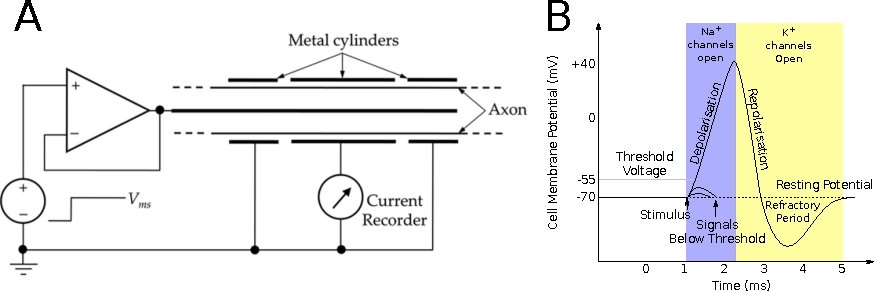
\includegraphics[width=0.5\textwidth]{figures/Hodgkin-Huxley_action_potential.pdf}
	\end{center}
	\captionsetup{singlelinecheck = false, justification=raggedright}
	\caption[The Action Potential is a Solution to the Hodkin-Huxley Model] {\textbf{The Action Potential is a Solution to the Hodgkin-Huxley Model }}{The shape of the action potential is a similar sight in many physiology textbooks. It was is in fact discovered as a result of the mathematical modelling of Hodgkin and Huxley hinting at the deep biophysics of ion channels won them the 1963 Noble Prize in medicine. This discovery is an excellent example of how deep theoretical insight can lead to predictable models of living systems \cite{hodgkin1952, hodgkin1952a, hodgkin1952b, hodgkin1952c, hodgkin1952d, hodgkin1952e}.}
	\label{action_potential_graphic}
\end{figure}

Similar to the above story, ion channels have always motivated the early pioneers of molecular biophysics. This is due to their ubiquity and importance in biological systems and the ease of measuring their activity with biochemical assays. One just needs an oscilloscope to measure their current. As cell biology has advanced it has become clear that the resting potential of a cell is critical to its function, regulating many chemical reactions inside it.

It's quite interesting that ion channels are the targets of comprise 19\% of approved drugs.\cite{santos2017} An exciting implication of this is the finesse with which we can now manipulate these systems in order to regulate morphogenesis in addition to the internal signalling environment of cells \cite{}. CITE Mike LEVIN.

These factors have to allowed biophysicists sufficient data to build sufficiently accurate models of biomolecular systems which generalise to other systems. Leading to a thriving field, analysing systems as diverse as protocells to gold nano particles CITATIONS NEEDED.

The discovery of voltage gated channels and a resting potential are still subjects studied in cell biology today as they are critical to the cells' function \cite{}.

So by using ion channels as basic biophysical laboratories have been used consistently to understand higher level protein physics \cite{}, and now we can apply this molecular understanding to attempt to tackle other diseases as experimental techniques have improved such as diabetes, and neurodegenerative diseases. Having an atomistic understanding is allowing us to study medicine with atomic precision.

%=======================================================================================%

\section{Studying Cystic Fibrosis is a an Opportunity to Learn biophysics and Treat disease.} 

The sad truth of this debilitating disease is that those afflicted are extremely unlucky. A single, change to the genome and their lungs fill with sticky mucus and become infected with bacteria, each breath cumbersome. Personally, I've not met somebody who has this disease. I have consistently wondered what perspective I'm missing by not suffering myself from such a condition or even knowing somebody with it. I'm not been trained in the ethics of studying medicine.

In this way, my motivations for studying this protein aren't solely focussed on treating disease. There is a perspective on protein evolution which states that the primary sequence of a particular gene contributes to the overall fitness of an organisms by a formula \cite{depristo2005a}.

\begin{equation}
	W(\Delta G) \propto \exp\bigg(\bigg[-\frac{\Delta G - \Delta G_{opt}}{\sigma_{\Delta G}}\bigg]^4\bigg) + c
\end{equation}

Where $W$ represents the fitness of the organism, $\Delta G$ is the folding energy of the protein and $\Delta G_{opt}$ is the folding energy of the protein . Figure \ref{fitness_landscape_gene_figure} demonstrates the types of random walks of a gene through sequence space which this model predicts. 

It just so happens that the CFTR gene sits at the precipice of a daunting cliff in sequence space. Where the band of stability in the modified gaussian in figure \ref{fitness_landscape_gene_figure} is extremely narrow. So by taking small steps in sequence space and plunging down this cliff we can try to understand how we might push the ball back up the cliff and retain functionality.

Moreover, by learning the nuts and bolts of what goes wrong with CFTR we can start to think about where some of these cliffs might be in other places in the proteome, to gain function and avoid disease and debilitation.

The reality of disease pathogenesis being caused by so many different mutations means that there has been decades of investigation into the function of every domain in the protein. 

This theoretical model is informs the conclusions of chapter \ref{chap:conclusions}.

Due to the array of disease causing mutations which occur accross the cystic fibrosis protein, there is a large body of literature on its unique function. This allows us a glance into its function and an opportunity to simultaneously perform basic biophysical research while directly assisting in furthering patient outcomes. This is the sort of inquiry which drives basic science forward, combining interesting experimental data into theoretical models to make testable predictions. The aim of this thesis is to build a model to make predictions about which kind of drugs will produce positive patient outcomes.

\section{Welcome to the Future}
Throughout science, the integration of experimental data with theoretical models leads to new and exciting research, this is particularly true in biology with its important applications in medicine, agriculture and increasingly, manufacturing. Wet lab biologists take advantage of experimental techniques which allow them to understand the dynamics and structure of living things from the top down. The finer the experimental instrument, the finer the detail they may resolve. Conversely, computational and theoretical biologists take a bottom up approach, we aim to take the granular details of a system, and integrate them upwards to model the macroscopic behaviour of that system. With more powerful computers and more detailed models we can make predictions about the behaviour of more complex systems. What is so exciting about the current era of biological research is that the domains of these two approaches are beginning to overlap, where they can synergize  and drive further breakthroughs. As we discover more systems where this overlap can be found we will develop more sophisticated treatments for diseases and problems found around the world.

The reason this has happened before in physics is two fold. Physical systems are much more homogeneous. So it's much easier to integrate upwards in length scale. Once you understand the pairwise interaction between two components it's simply a question of having the theoretical and computational capacity to model the bulk behaviour of that system. 

The difference with biological systems is that they have so many different components that finding an analytic or even computationally tractable solution is usually impossible. However, as we collect more data and build more powerful computers we can approach more complete models. These in turn inform more powerful theoretical models these help direct the material efforts of experimental expertise . 

While previously we were limited it functional data concerning ion channels we now have unprecedented resolution for the structure dynamics for the inside of a cell. Advances in cryogenic electron microscopy, confocal microscopy, X-ray Crystallography, fluorescent microscopy and genetic engineering allow us to glimpse unprecendented information about the salty dance of life inside cells.

Alphafold is a good example. This new breakthrough builds on decades of inquiry from the structural biology community and advancements in AI to give high resolution protein structures. Now this result can be used to fill in the gaps of structural biology. Crucually, alphafold konws what it doesn't know. So we can tell where to direct the efforts of structural biology. Together these advances will fill more gaps in our knowledge of protein physics. 

Armed with this philosophy we will delineate how to use the causal unit of the Schr\"oedinger wave equation to make approximations to atomic systems in order to create a biophysical model for macromolecular systmes like proteins.
